\label{s:animated-transitions-implemented}
The implemented animated transitions between visual appearances are shown in Table \ref{tab:transition-table-implemented} on page \pageref{tab:transition-table-implemented}. Every transition is described with abbreviations in the table which are explained in detail in the description list below. A cell containing several abbreviations denotes the transition flow step by step. Thus, the list consists of basic transitions which are combined in various ways in order to achieve an animated transition from one visualisation type to another one.

\begin{description}
\item[Area-colour] \hfill \\
Colouring enumeration units where the colour either is determined by the current selected colour scheme or the default colour.

\item[CB-colour] \hfill \\
Centroid-based colouring is only used in conjunction the \textit{Draw default}-transition. Particles moving to its centroid colour their appropriate symbol when reaching the centroid.

\item[Draw defaults] \hfill \\
Default symbols (circles) are drawn for each enumeration unit at its centroid. Each circle has a default radius. This transition state is mainly used to set up following ones.

\item[Force] \hfill \\
This transition state is only used to create cartograms. Force is dependent on symbols in the screen. It applies collision detection and gravity on those symbols in order to create the Pseudo-Demers cartogram.

\item[Origin-colour] \hfill \\
Origin-colour is the exact opposite of "CB-Colour. All particles are moving from their centroid to their origin location. When leaving their appropriate symbol, the colour of the symbol adapts accordingly.

\item[Scale] \hfill \\
Scaling is also dependent on existing symbols. When scaling is triggered, all symbols are either scaled to their population or back to a default value.

\item[Symbol-colour] \hfill \\
All symbols are coloured at once appropriately to their amount of orders.

\item[Symbol-translation] \hfill \\
If the current visualisation is a cartogram and the user wishes to change the visual appearance, all symbols need to move back to their origin again.

\end{description}

\begin{table}[!htp]
    \begin{tabular}{M{27mm}|| M{27mm} | M{27mm} | M{27mm} | M{27mm} N}

    ~ & Dot Map & Proportional Symbol Map & Choropleth Map & Cartogram &\\[4ex] \hline \hline

    Dot Map & ~ & Scale, Origin-colour & Draw defaults, Area-colour, Symbol-colour, Origin-colour & Symbol-translation, Scale, Origin-colour &\\[4ex] \hline

    Proportional Symbol Map & Draw defaults, CB-colour, Scale & ~ & Draw defaults, Area-colour, Symbol-colour, Scale & Symbol-translation &\\[4ex] \hline

    Choropleth Map & Draw defaults, CB-colour, Area-colour & Scale, Area-colour & ~ & Symbol-translation, Scale, Area-colour &\\[4ex] \hline

    Cartogram & Draw defaults, CB-colour, Scale, Force & Force & Draw defaults, Area-colour, Symbol-colour, Scale, Force & ~ &\\[4ex]

    \end{tabular}
    \caption{Transition table showing the implemented transition from a given visualisation (column) to any upcoming visualisation (rows)}
    \label{tab:transition-table-implemented}
\end{table}

The implemented web application is accessible online\footnote{See \href{https://particles-masterthesis.github.io/aggregation/}{https://particles-masterthesis.github.io/aggregation/} for more information.}. The following Figures featured in this Section are all taken directly from application. The source code is also accessible online\footnote{See \href{https://github.com/particles-masterthesis/aggregation}{https://github.com/particles-masterthesis/aggregation} for more information.}.

The implemented application only features basic interaction methods. Figure \ref{f:showcase-overall} on page \pageref{f:showcase-overall} shows a navigation bar and the configurable settings. Changing the visual appearance can be achieved by interacting with the bar. If changing any kind of configuration is desired, e.g. the speed of moving particles or the level of detail shown, this can be done by using the graphical user interface in the top right.

\begin{figure}[!htb]

   \begin{minipage}{\linewidth} 
        \centering
        \subcaptionbox
        [
            Particle-based dot map        
        ]
        {
            Particle-based dot map.
            \label{f:showcase-dot}
        }
        [.4\linewidth]
        {
            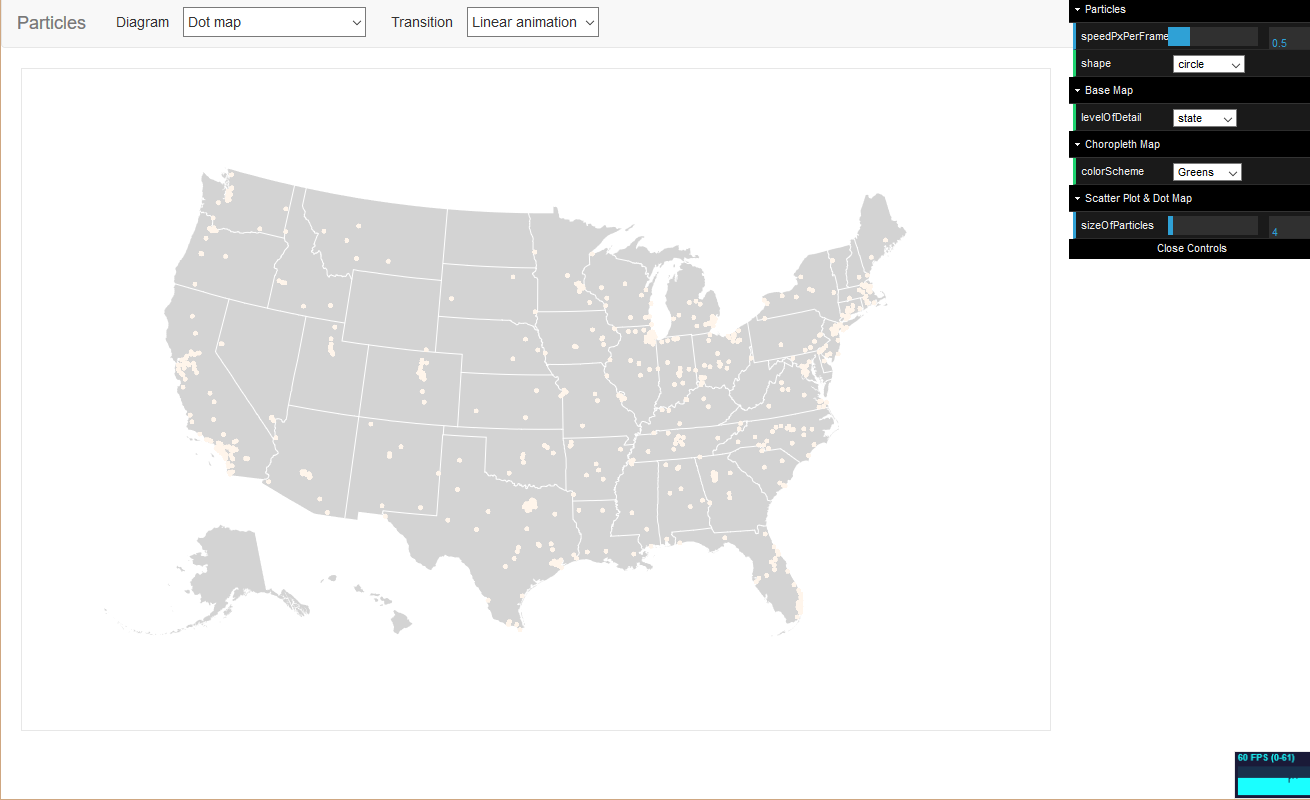
\includegraphics[width=0.4\textwidth,keepaspectratio]
            {images/results/map_dot.png}
        }
        \qquad
        \subcaptionbox
        [
          Multivariate classed proportional symbol map
        ]
        {
            Multivariate classed proportional symbol map
            \label{f:showcase-psm}
        }
        [.4\linewidth]
        {
            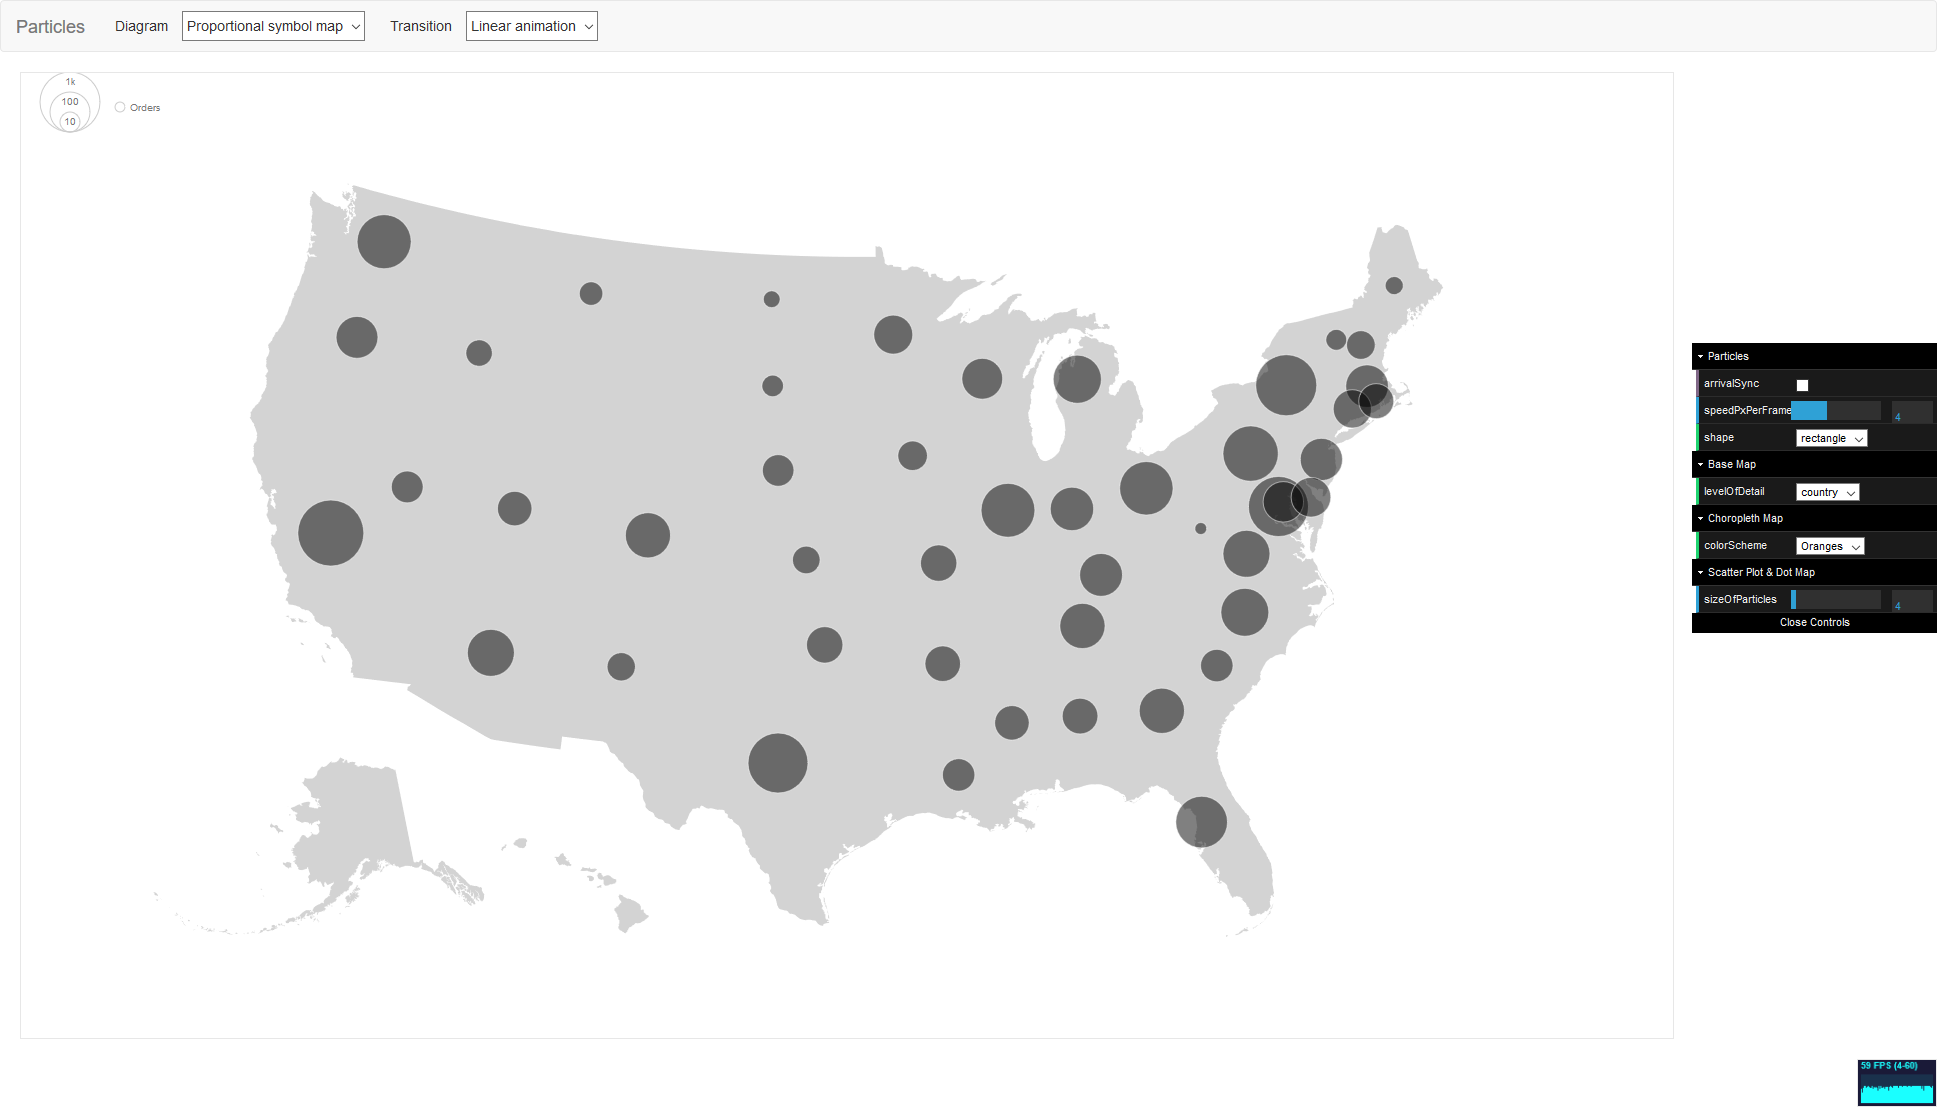
\includegraphics[width=0.4\textwidth,keepaspectratio]
            {images/results/map_psm.png}
        }
   \end{minipage} 

   \begin{minipage}{\linewidth} 
        \centering
        \subcaptionbox
        [
            Classed choropleth map.
        ]
        {
            Classed choropleth map.
            \label{f:showcase-choropleth}
        }
        [.4\linewidth]
        {
            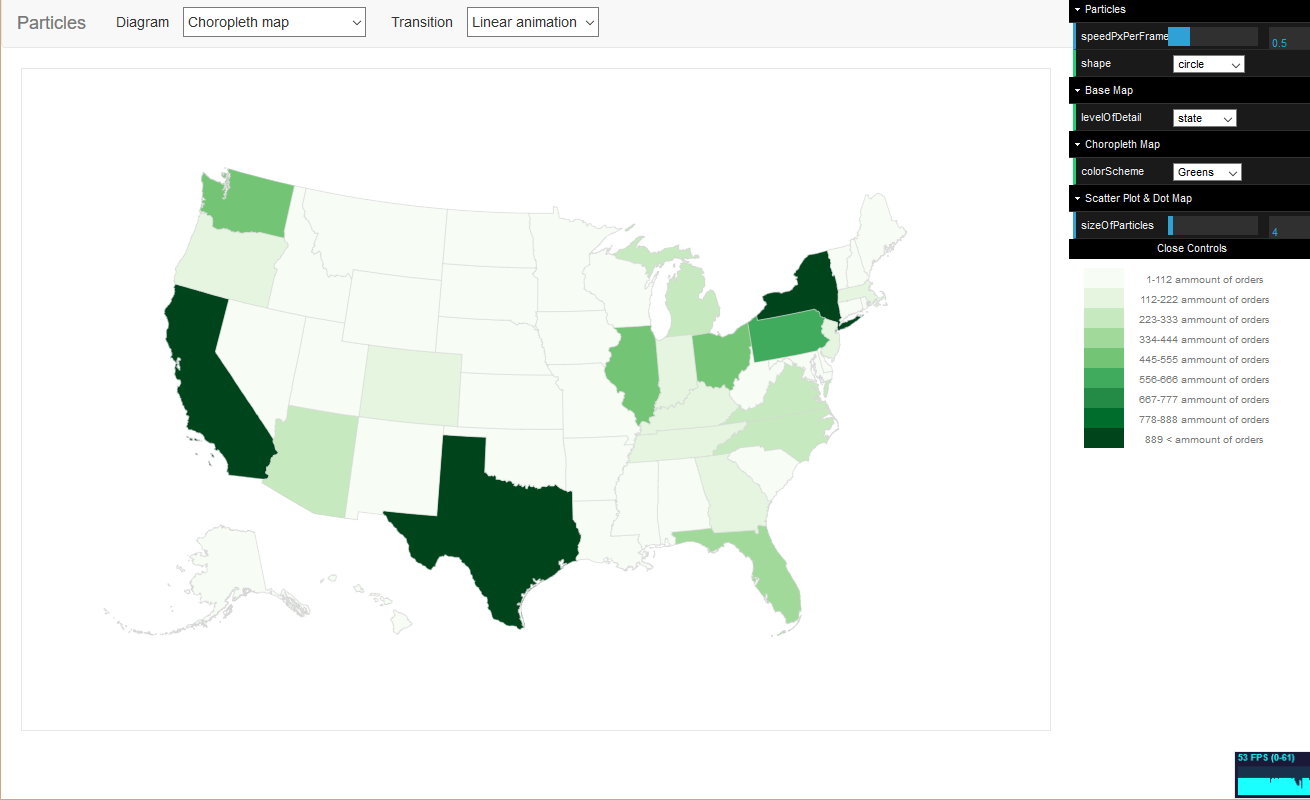
\includegraphics[width=0.4\textwidth,keepaspectratio]
            {images/results/map_choropleth.png}
        }
        \qquad
        \subcaptionbox
        [
          Classed Pseudo-Demers cartogram.
        ]
        {
            Classed Pseudo-Demers cartogram
            \label{f:showcase-cartogram}
        }
        [.4\linewidth]
        {
            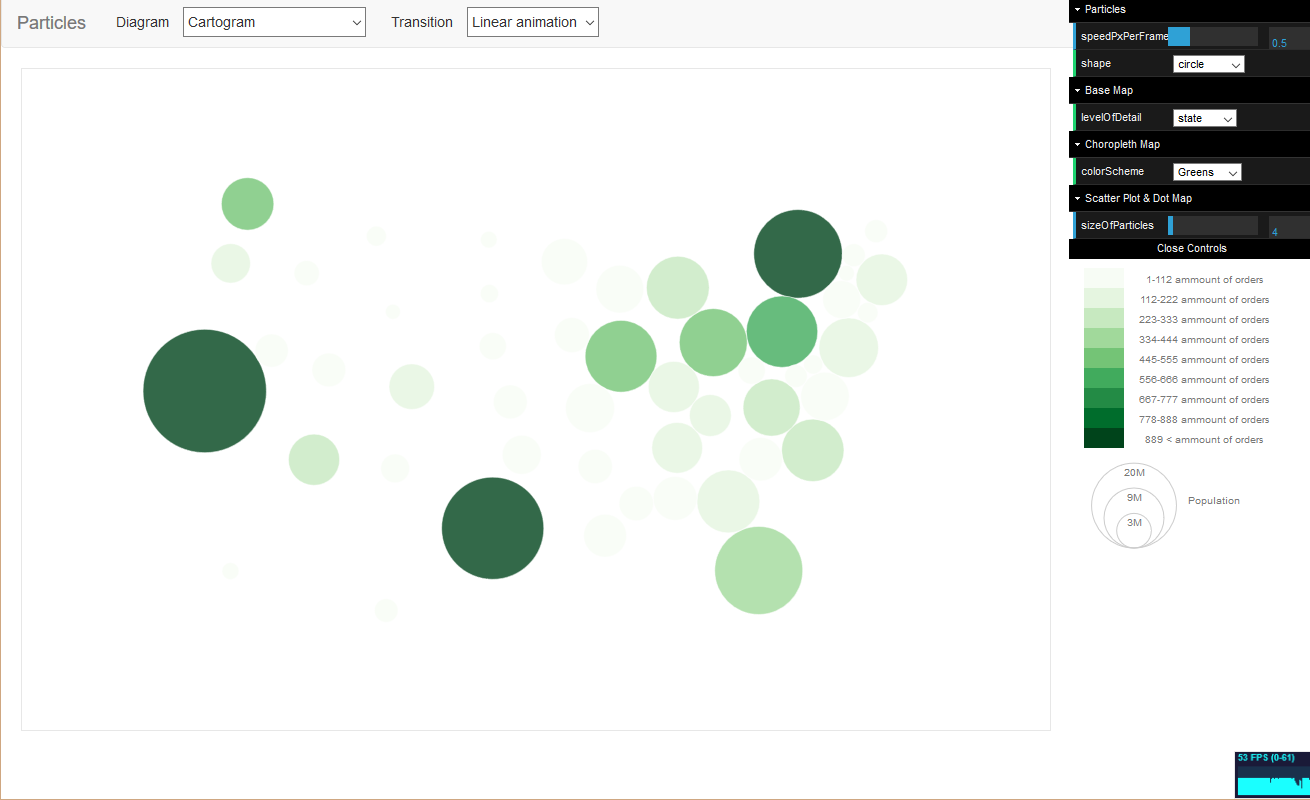
\includegraphics[width=0.4\textwidth,keepaspectratio]
            {images/results/map_cartogram.png}
        }
   \end{minipage} 
    \caption[The implemented web-application showing four different types of geo-spatial map visualisations and with its interaction possibilities.]
    {The implemented web-application showing four different types of geo-spatial map visualisations and with its interaction possibilities.}
    \label{f:showcase-overall}
\end{figure}



Furthermore, Figure \ref{f:showcase-overall} on page \pageref{f:showcase-overall} shows the implemented geo-spatial map visualisations. Figure \ref{f:showcase-dot} shows the implemented dot map, \ref{f:showcase-psm} the multivariate classed proportional symbol map, \ref{f:showcase-choropleth} the classed choropleth map and \ref{f:showcase-cartogram} the classed Pseude-Demers cartogram.

One herein before mentioned animated transition is showcased in Figure \ref{f:showcase-transition-dot-cartogram} on page \pageref{f:showcase-transition-dot-cartogram}. It shows the animated transition from the dot map to the Pseudo-Demers cartogram. Table \ref{tab:transition-table-implemented} on page \pageref{tab:transition-table-implemented} explaines the stacked transitions in detail. The Figure needs to be read line by line. The level of detail in the example is set to use state-data. Step 1 shows the dot map which is the starting point of the transition. Step 2 illustrates the default symbols (Draw defaults). Step 3 to 5 are showing the CB-colour transition where all particles are moving to their appropriate centroid and colouring it if they reach their destination. If this transition is finished, step 6 and 7 show the scaling of the symbols according to their population. Step 8 displays the force which is applied in case of a collision and the remaining subfigures showcase the location preserable gravity applied to each symbol. If the transition is entirely finished, the base map is removed.

\begin{figure*}
    \centering

    \begin{subfigure}[b]{0.31\textwidth}
        \centering
        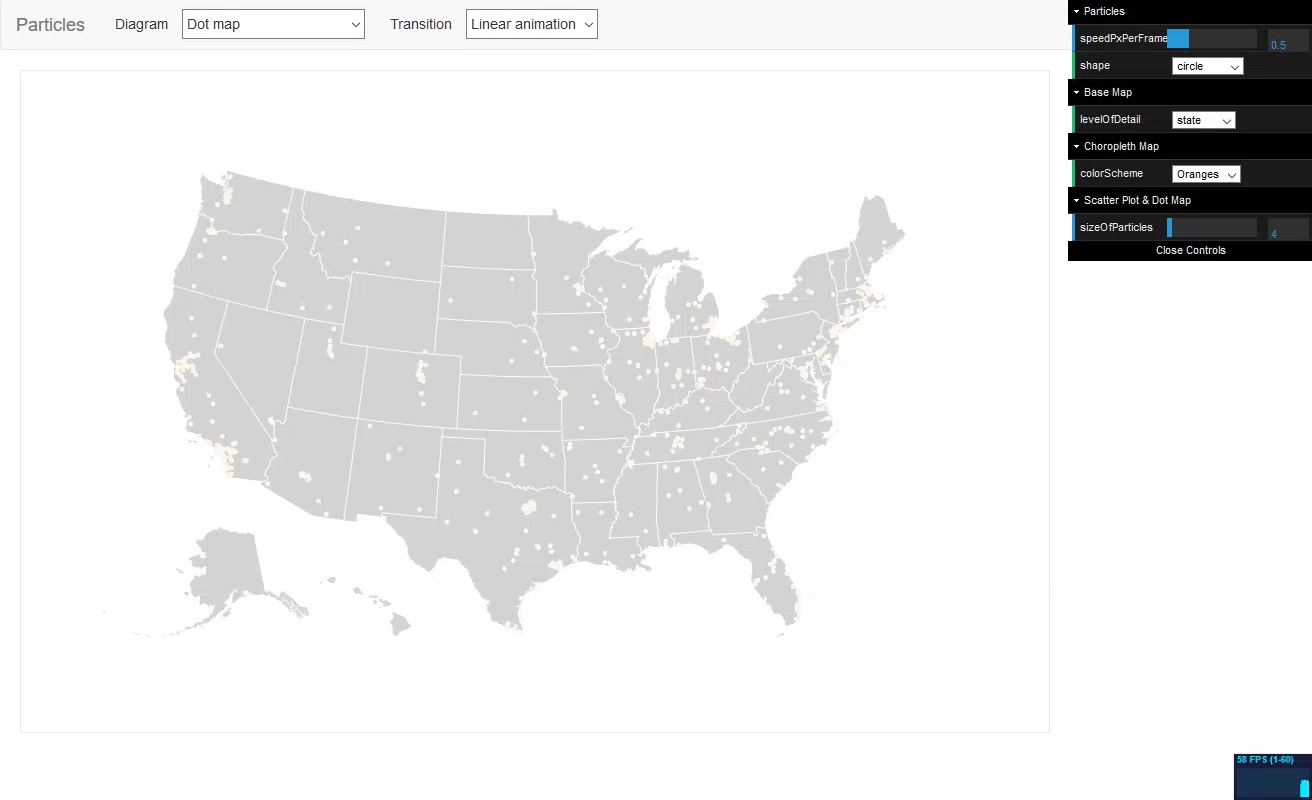
\includegraphics[width=\textwidth]{images/results/dot_cartogram/transition_1.png}
        \caption[]%
        {{\small Step 1}}
    \end{subfigure}
    \hfill
    \begin{subfigure}[b]{0.31\textwidth}
        \centering
        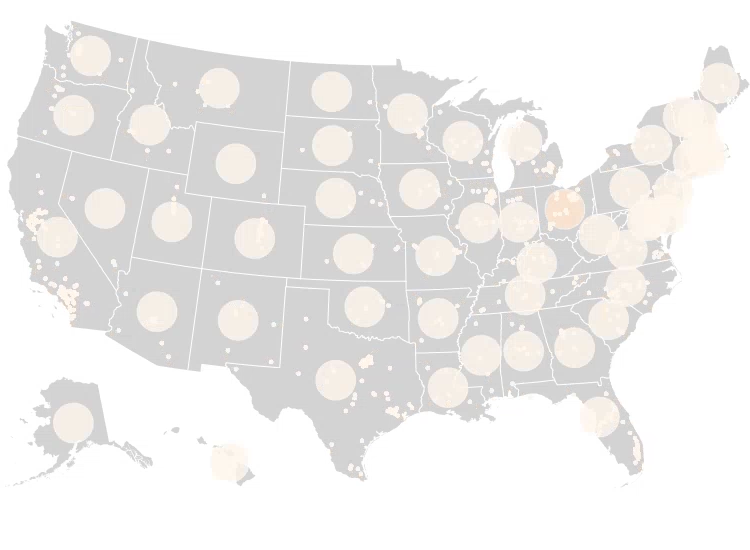
\includegraphics[width=\textwidth]{images/results/dot_cartogram/transition_2.png}
        \caption[]%
        {{\small Step 2}}
    \end{subfigure}
    \hfill
    \begin{subfigure}[b]{0.31\textwidth}
        \centering
        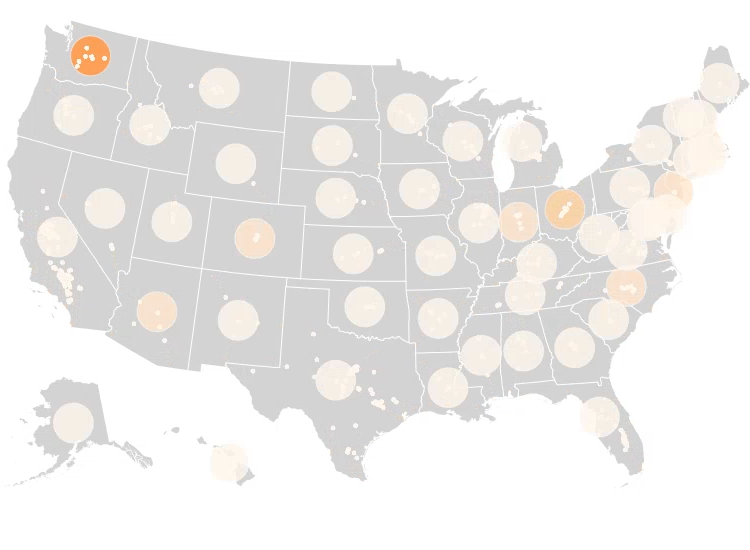
\includegraphics[width=\textwidth]{images/results/dot_cartogram/transition_3.png}
        \caption[]%
        {{\small Step 3}}
    \end{subfigure}
    \vskip\baselineskip

    \begin{subfigure}[b]{0.31\textwidth}
        \centering
        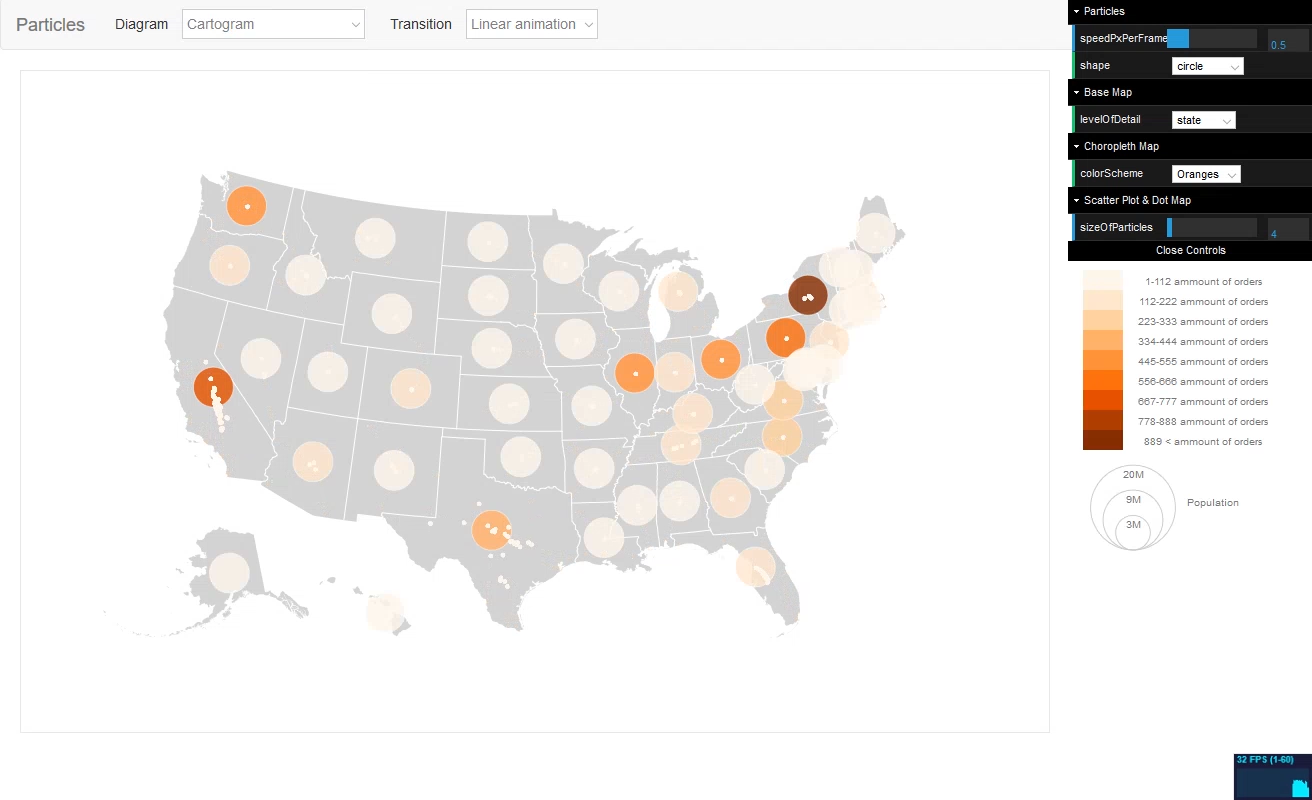
\includegraphics[width=\textwidth]{images/results/dot_cartogram/transition_4.png}
        \caption[]%
        {{\small Step 4}}
    \end{subfigure}
    \hfill
    \begin{subfigure}[b]{0.31\textwidth}
        \centering
        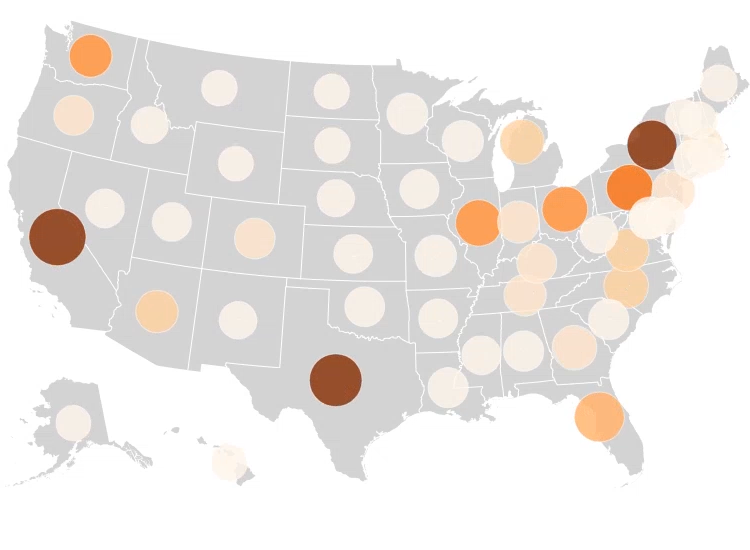
\includegraphics[width=\textwidth]{images/results/dot_cartogram/transition_5.png}
        \caption[]%
        {{\small Step 5}}
    \end{subfigure}
    \hfill
    \begin{subfigure}[b]{0.31\textwidth}
        \centering
        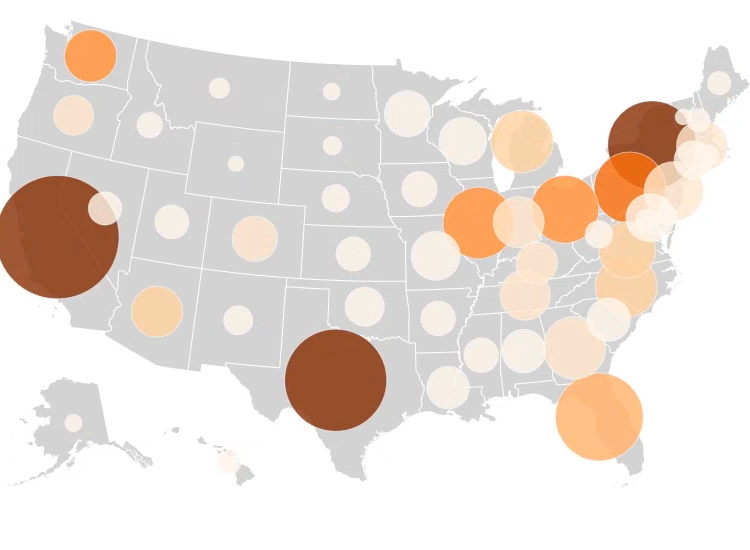
\includegraphics[width=\textwidth]{images/results/dot_cartogram/transition_6.png}
        \caption[]%
        {{\small Step 6}}
    \end{subfigure}
    \vskip\baselineskip

    \begin{subfigure}[b]{0.31\textwidth}
        \centering
        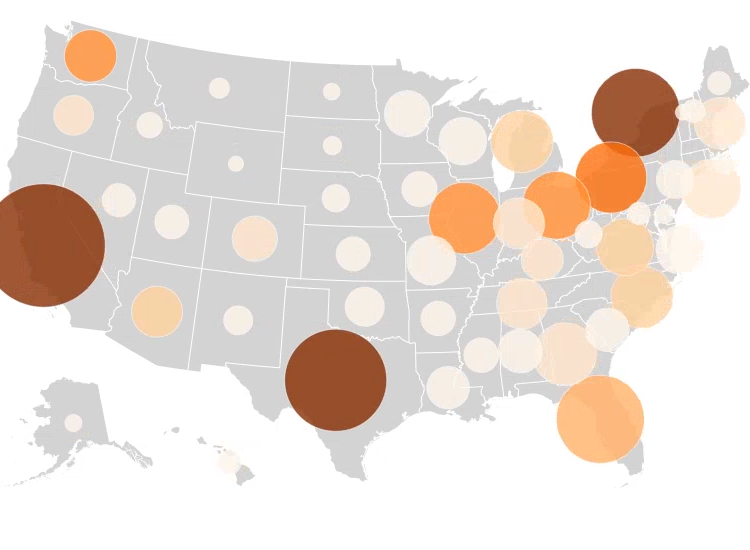
\includegraphics[width=\textwidth]{images/results/dot_cartogram/transition_7.png}
        \caption[]%
        {{\small Step 7}}
    \end{subfigure}
    \hfill
    \begin{subfigure}[b]{0.31\textwidth}
        \centering
        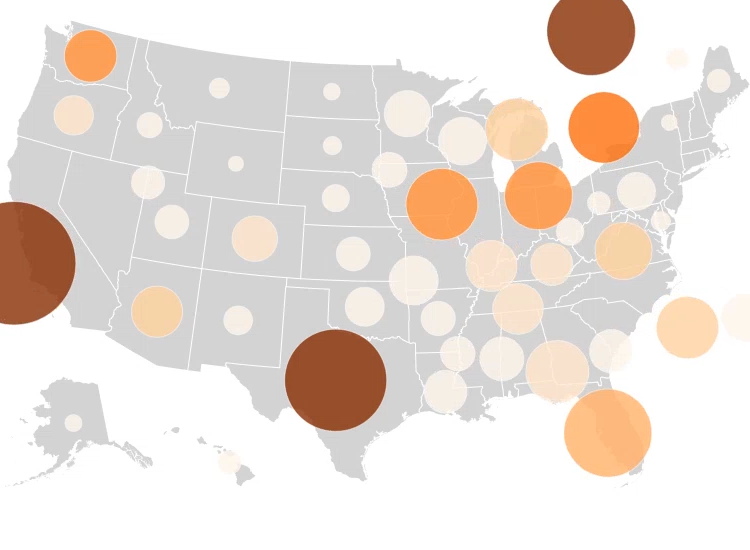
\includegraphics[width=\textwidth]{images/results/dot_cartogram/transition_8.png}
        \caption[]%
        {{\small Step 8}}
    \end{subfigure}
    \hfill
    \begin{subfigure}[b]{0.31\textwidth}
        \centering
        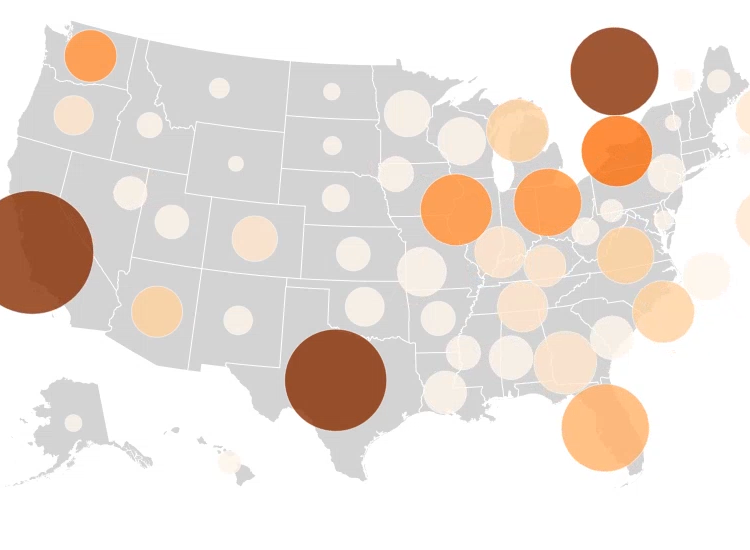
\includegraphics[width=\textwidth]{images/results/dot_cartogram/transition_9.png}
        \caption[]%
        {{\small Step 9}}
    \end{subfigure}
    \vskip\baselineskip

    \begin{subfigure}[b]{0.31\textwidth}
        \centering
        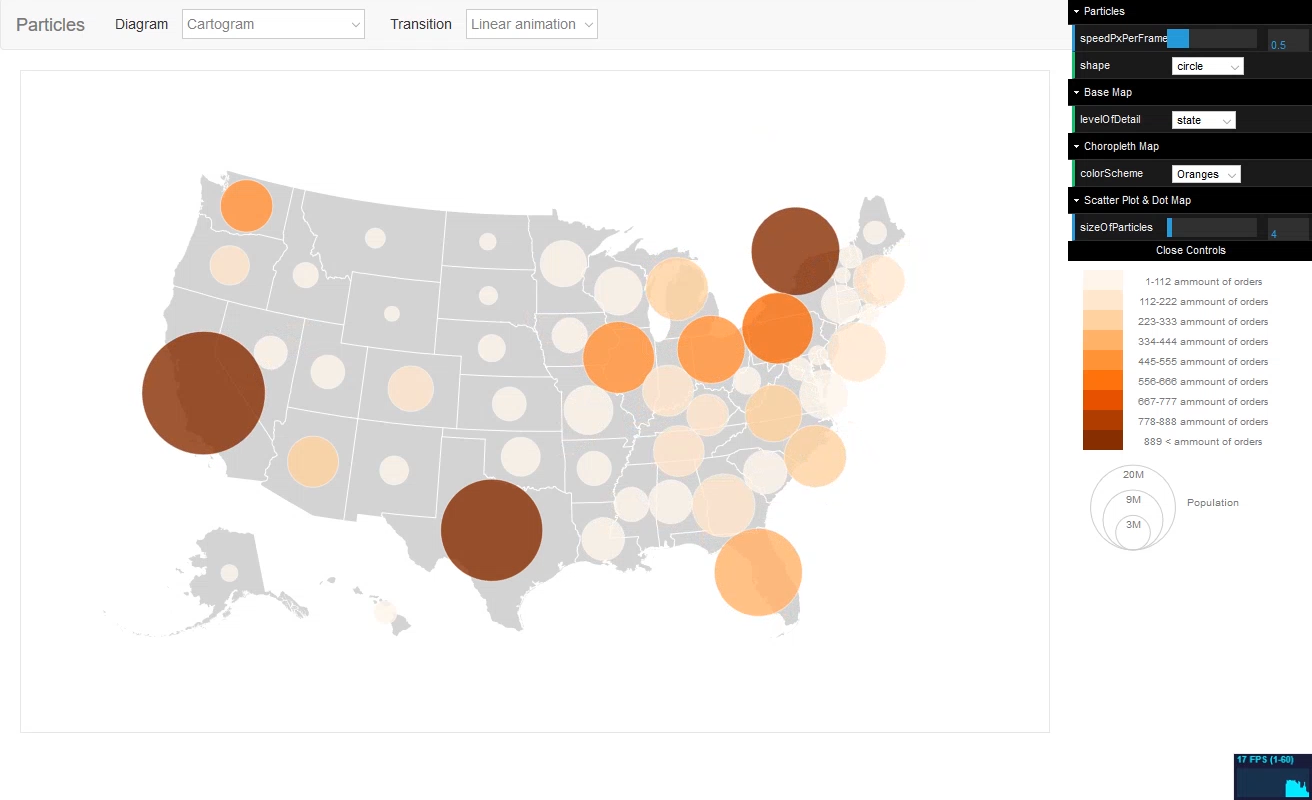
\includegraphics[width=\textwidth]{images/results/dot_cartogram/transition_10.png}
        \caption[]%
        {{\small Step 10}}
    \end{subfigure}
    \hfill
    \begin{subfigure}[b]{0.31\textwidth}
        \centering
        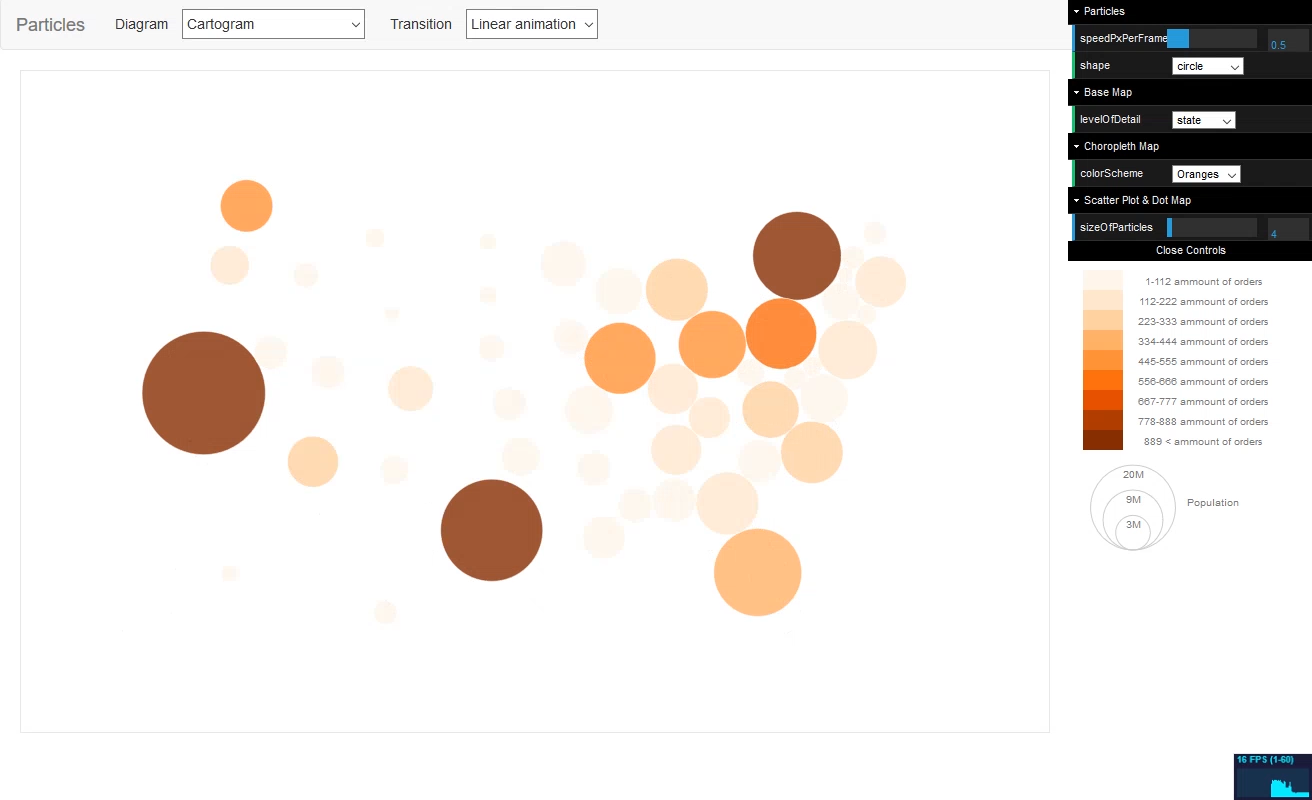
\includegraphics[width=\textwidth]{images/results/dot_cartogram/transition_11.png}
        \caption[]%
        {{\small Step 11}}
    \end{subfigure}
    \hfill
    \begin{subfigure}[b]{0.31\textwidth}
        \centering
        
\includegraphics[width=\textwidth]{images/results/dot_cartogram/transition_12.png}
    \end{subfigure}
    \vskip\baselineskip

    \caption[Showcase of the implemented animated transition from a dot map to the Pseudo-Demers cartogram]
    {\small Showcase of the implemented animated transition from a dot map to the Pseudo-Demers cartogram}
    \label{f:showcase-transition-dot-cartogram}
\end{figure*}
